\subsection{Population Generation}

The population generator will, as the name suggests, populate the terrain provided as input. Specifically, a heat map will be generated in the background of the terrain which will represent the population density for the entire plane.
The heat map is given by the noise module, and this invisible heat map can be brought forth within debug mode.
The areas of high density population can be altered with user input.
When generating the population map, the user will get a visual option to choose a location for a city, which is a point on the terrain of which the radius can also be customized.
On this marker, the population density of that area will be drastically increased.

The population generator was responsible for creating a procedurally generated intensity map describing the population in the world.
High intensity areas meant that there was a higher density of the population.
Multiple generators in the sequence required a population map to create more realistic buildings, thus the population map needed to reflect the landscape accordingly.
Because of that, the population map was responsible for the rough shape of the city.

To generate an intensity map, it required the terrain parameter, which was used to mask off certain areas in the landscape, such as oceans, rivers or mountains.
Then, the generator would use a few layers of simplex noise to create a representation of populations throughout the world.
Population markers were used to increase population density in a certain area, and these were applied after generating the initial population map.
This was useful for making sure the center of cities have a higher density, but it would still respect the original population map to some degree.
In figure 4.2, a population marker was placed in the center of the city, which meant the population density was much higher there.
White areas have a higher population density, dark areas have a lower population density. This figure also shows that main roads outside the cities will tend to shy away from lower-density areas, but not always.

\begin{figure}[h!]
  \centering

  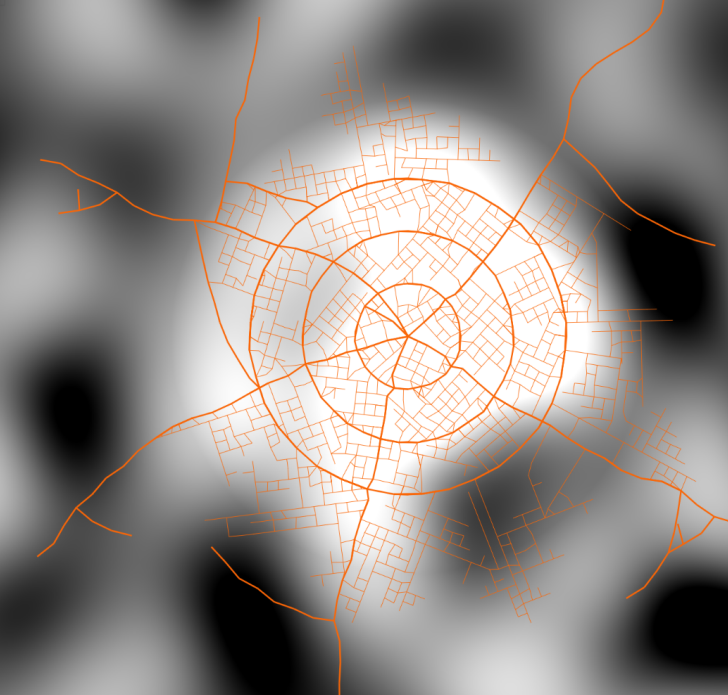
\includegraphics[width=0.8\textwidth]{figure/pop_density.png}
  \caption{An example of a population map with a Paris city generated within it.}

  \label{fig:population density}
\end{figure}